\documentclass[12pt,letterpaper]{article}

\usepackage[utf8]{inputenc}
\usepackage[T1]{fontenc}
\usepackage[spanish,es-nodecimaldot]{babel}
\usepackage{lmodern}
\usepackage{geometry}
\usepackage{microtype}
\usepackage{graphicx}
\usepackage{booktabs}
\usepackage{tabularx}
\usepackage{array}
\usepackage{longtable}
\usepackage{amsmath}
\usepackage{xcolor}
\usepackage{float}
\usepackage{enumitem}
\usepackage{listings}
\usepackage{fancyhdr}
\usepackage{titlesec}
\usepackage[hidelinks]{hyperref}
\hypersetup{
  pdftitle={Transformada Lineal de Hough con CUDA},
  pdfauthor={Pablo Daniel Barillas Moreno y Milton Giovanni Polanco Serrano},
  pdfsubject={Proyecto 3 de Computación Paralela y Distribuida}
}

\geometry{top=2.3cm,bottom=2.3cm,left=2.6cm,right=2.6cm}
\setlength{\parindent}{0pt}
\setlength{\parskip}{0.65em}
\renewcommand{\arraystretch}{1.18}
\setlist{itemsep=0.25em,topsep=0.25em}

\definecolor{uvgblue}{HTML}{0B3954}
\definecolor{uvgteal}{HTML}{087E8B}
\definecolor{uvgpurple}{HTML}{6D28D9}
\definecolor{uvgorange}{HTML}{D95F02}
\definecolor{codebg}{HTML}{F3F6F8}

\titleformat{\section}{\Large\bfseries\color{uvgblue}}{\thesection.}{0.6em}{}
\titleformat{\subsection}{\large\bfseries\color{uvgteal}}{\thesubsection.}{0.6em}{}

\pagestyle{fancy}
\fancyhf{}
\fancyhead[L]{Transformada Lineal de Hough con CUDA}
\fancyhead[R]{Grupo 1 - Sección 40}
\fancyfoot[C]{\thepage}
\setlength{\headheight}{14.5pt}
\renewcommand{\headrulewidth}{0.4pt}

\lstset{
  language=C++,
  backgroundcolor=\color{codebg},
  basicstyle=\ttfamily\small,
  keywordstyle=\color{uvgpurple}\bfseries,
  commentstyle=\color{uvgteal},
  stringstyle=\color{uvgorange},
  frame=single,
  rulecolor=\color{black!15},
  breaklines=true,
  columns=fullflexible,
  showstringspaces=false
}

\newcommand{\carnePablo}{22193}
\newcommand{\carneMilton}{23471}

\begin{document}
\pagenumbering{gobble}

\begin{titlepage}
  \centering
  \vspace*{1.2cm}
  {\Large\bfseries Universidad del Valle de Guatemala\par}
  \vspace{0.4cm}
  {\large Computación Paralela y Distribuida\par}
  {\large Docente: Sebastián Galindo\par}
  \vfill
  {\color{uvgblue}\rule{\textwidth}{1.2pt}\par}
  \vspace{0.7cm}
  {\Huge\bfseries Transformada Lineal de Hough con CUDA\par}
  \vspace{0.35cm}
  {\Large Memoria Global, Constante y Compartida\par}
  \vspace{0.7cm}
  {\color{uvgblue}\rule{\textwidth}{1.2pt}\par}
  \vfill
  \begin{tabular}{rl}
    \textbf{Grupo:} & 1 \\
    \textbf{Sección:} & 40 \\
    \textbf{Integrante:} & Pablo Daniel Barillas Moreno \\
    \textbf{Carné:} & \carnePablo \\
    \textbf{Integrante:} & Milton Giovanni Polanco Serrano \\
    \textbf{Carné:} & \carneMilton \\
  \end{tabular}
  \vfill
  {\large Guatemala, 7 de noviembre de 2026\par}
\end{titlepage}

\pagenumbering{roman}
\tableofcontents
\listoffigures
\listoftables
\clearpage
\pagenumbering{arabic}

\section{Introducción}

Las unidades de procesamiento gráfico permiten ejecutar miles de hilos concurrentes, pero el paralelismo por sí solo no garantiza una mejora de rendimiento. La ubicación de los datos, el patrón de acceso, la sincronización y la contención de las operaciones atómicas también influyen en el tiempo de ejecución \cite{cuda-guide}. Este proyecto estudia esos efectos con la versión lineal de la Transformada de Hough, un algoritmo de visión por computadora que detecta rectas mediante un sistema de votación geométrica \cite{duda-hart}.

Se implementaron tres versiones CUDA. La primera almacena la imagen, las tablas trigonométricas y el acumulador en memoria global. La segunda traslada las tablas de seno y coseno a memoria constante. La tercera añade un acumulador parcial en memoria compartida para cada bloque y luego fusiona sus resultados con el acumulador global. Las tres versiones utilizan la misma imagen, discretización y geometría para permitir una comparación controlada.

El programa también genera una imagen PNG con las líneas detectadas, conserva los tiempos y parámetros en archivos CSV y compara los 9,000 bins de cada variante contra una referencia CPU.

\section{Fundamento de la Transformada de Hough}

Una recta puede representarse mediante su distancia perpendicular al origen, $r$, y el ángulo de su normal, $\theta$:

\begin{equation}
  r = x\cos(\theta) + y\sin(\theta).
  \label{eq:hough}
\end{equation}

Cada píxel activo $(x,y)$ vota por todas las rectas que podrían contenerlo. El programa discretiza $\theta$ entre 0 y 178 grados, con incrementos de 2 grados, para obtener 90 bins angulares. El rango radial $[-r_{\max},r_{\max}]$ se divide en 100 bins. El acumulador contiene entonces $90\times100=9{,}000$ contadores. Los máximos representan las rectas más respaldadas por la imagen.

La imagen tiene su origen en la esquina superior izquierda. El kernel traslada ese origen al centro e invierte el eje vertical:

\begin{lstlisting}
int x_coordinate = global_id % width - width / 2;
int y_coordinate = height / 2 - global_id / width;
\end{lstlisting}

El módulo obtiene la columna y la división entera obtiene la fila. La resta horizontal centra el eje $x$. La resta vertical invierte la dirección porque las filas crecen hacia abajo, mientras que el eje cartesiano $y$ crece hacia arriba.

\section{Diseño de la implementación}

El grid asigna un hilo CUDA por píxel. El identificador lineal se calcula a partir del bloque y del hilo:

\begin{lstlisting}
int global_id = blockIdx.x * blockDim.x + threadIdx.x;
\end{lstlisting}

Cada hilo dentro de la imagen lee un píxel. Si su intensidad no supera el umbral, no emite votos. En caso contrario recorre los 90 ángulos, evalúa la ecuación~\ref{eq:hough}, discretiza $r$ y actualiza el bin correspondiente. Las actualizaciones concurrentes utilizan \texttt{atomicAdd} para impedir que dos hilos pierdan votos al escribir simultáneamente.

La referencia CPU usa las mismas tablas \texttt{float}, la misma discretización y el mismo redondeo. Después de medir cada variante se copian los 9,000 bins al host y se exige igualdad exacta. Ante cualquier diferencia, la ejecución informa el primer bin incorrecto y rechaza la corrida.

La aplicación utiliza RAII para liberar buffers y eventos cuando salen de alcance, comprueba los códigos de error de CUDA y ejecuta \texttt{cudaDeviceReset} al finalizar. La escritura PNG es autocontenida y no requiere OpenCV.

\section{Versión con memoria Global}

La versión base mantiene la imagen, las tablas trigonométricas y el acumulador en memoria global. Cada hilo consulta 90 valores de seno y coseno y registra 90 posibles votos si el píxel está activo. Todos los bloques comparten el mismo acumulador, de modo que varios hilos pueden intentar incrementar el mismo bin.

Esta estrategia ofrece una referencia simple y funcional. Su principal limitación es la contención causada por una gran cantidad de operaciones atómicas sobre memoria global. La variante Global sirve como línea base para calcular el speedup de las otras versiones.

\section{Aplicación de memoria Constante}

Las tablas contienen 90 senos y 90 cosenos de tipo \texttt{float}. En total ocupan 720 bytes, no cambian durante el kernel y todos los hilos de un warp consultan la misma posición durante una iteración angular. Estas propiedades encajan con el uso de memoria constante y su capacidad de distribuir una lectura uniforme mediante broadcast \cite{cuda-guide}.

\begin{lstlisting}
__constant__ float c_cos[90];
__constant__ float c_sin[90];

cudaMemcpyToSymbol(c_cos, cos_table.data(), cos_table.size() * sizeof(float));
cudaMemcpyToSymbol(c_sin, sin_table.data(), sin_table.size() * sizeof(float));
\end{lstlisting}

La imagen y el acumulador permanecen en memoria global. Por ello, la variante Constante reduce el costo potencial de consultar las tablas, pero no elimina la contención del acumulador.

\begin{figure}[H]
  \centering
  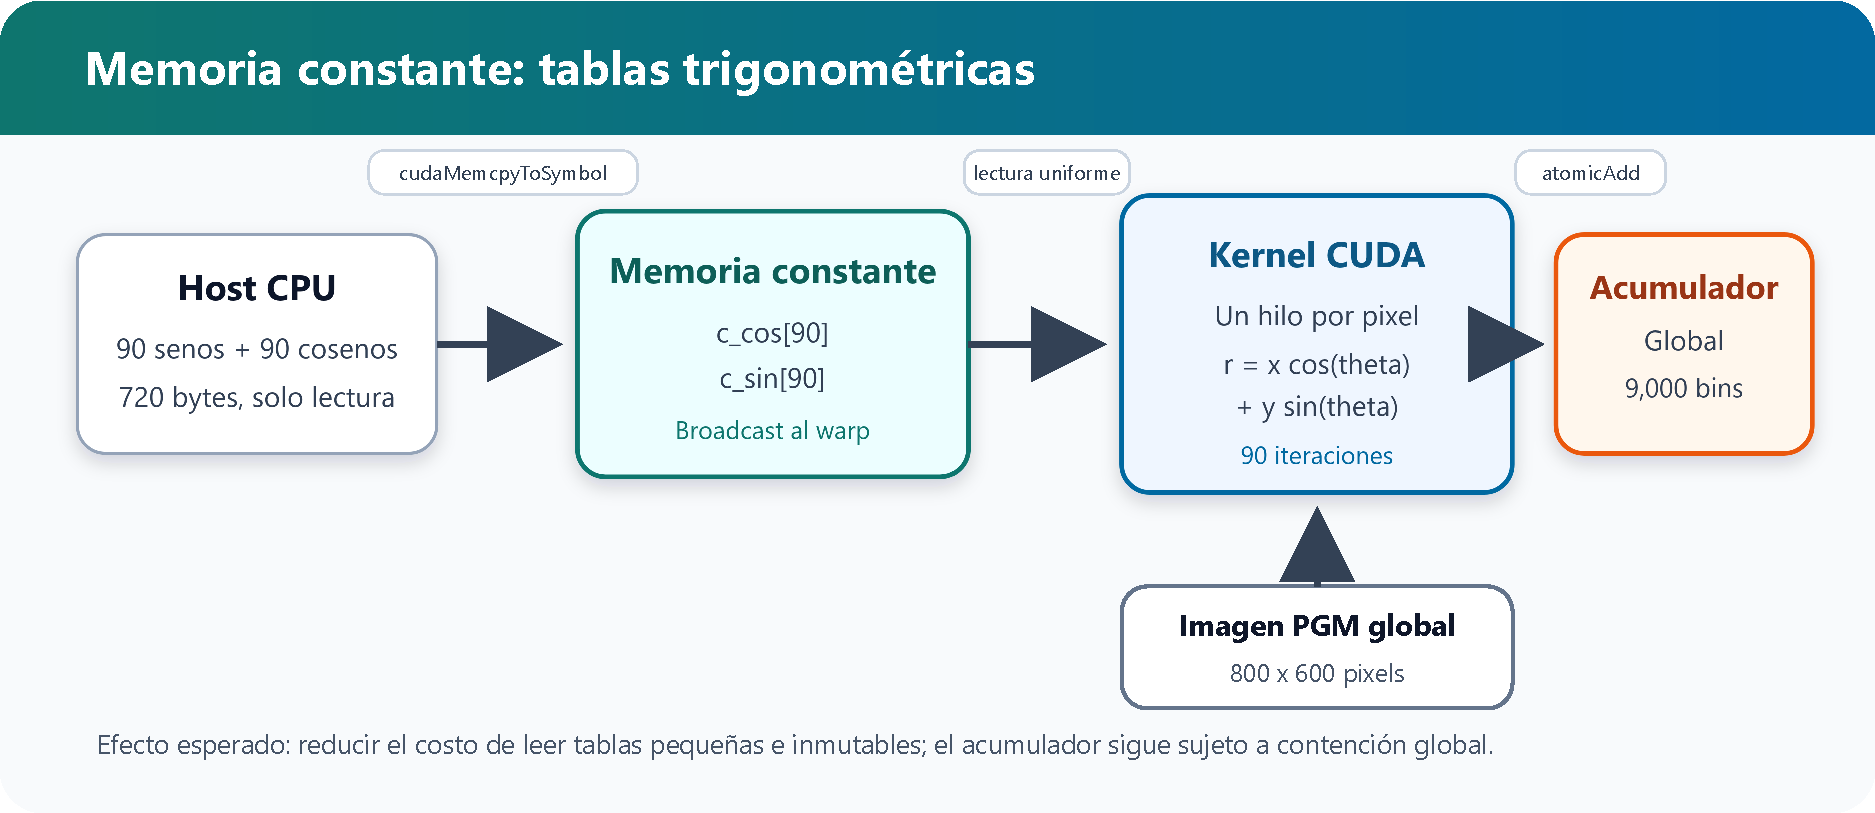
\includegraphics[width=\textwidth]{figures/memoria_constante.pdf}
  \caption{Uso de memoria constante para las tablas trigonométricas.}
  \label{fig:constant}
\end{figure}

La mejora esperada puede ser pequeña. Las tablas son compactas y otras cachés también pueden atender sus lecturas. Si las operaciones atómicas dominan el tiempo, optimizar 720 bytes de tablas produce un impacto limitado.

\section{Aplicación de memoria Compartida}

Cada bloque reserva un acumulador local de 9,000 enteros, equivalente a 36,000 bytes. Los 256 hilos cooperan para inicializarlo usando un bucle con paso \texttt{blockDim.x}. Una primera barrera garantiza que todos los bins estén en cero antes de votar.

Los votos se acumulan con operaciones atómicas en memoria compartida. Una segunda barrera garantiza que ningún hilo continúe a la fusión mientras otro aún vota. Finalmente, los hilos recorren cooperativamente el acumulador local y suman los bins no nulos al acumulador global.

\noindent\begin{minipage}{\linewidth}
\begin{lstlisting}
__shared__ int local_accumulator[kAccumulatorSize];
for (int index = local_id; index < kAccumulatorSize; index += blockDim.x)
    local_accumulator[index] = 0;
__syncthreads();
// Votacion con atomicAdd sobre local_accumulator.
__syncthreads();
for (int index = local_id; index < kAccumulatorSize; index += blockDim.x) {
    const int block_votes = local_accumulator[index];
    if (block_votes != 0) atomicAdd(&accumulator[index], block_votes);
}
\end{lstlisting}
\end{minipage}

Los hilos sobrantes del último bloque no retornan antes de las barreras. Solo omiten la votación y continúan participando en ambas sincronizaciones. Retornar antes de una barrera podría bloquear el bloque o producir comportamiento indefinido.

\begin{figure}[H]
  \centering
  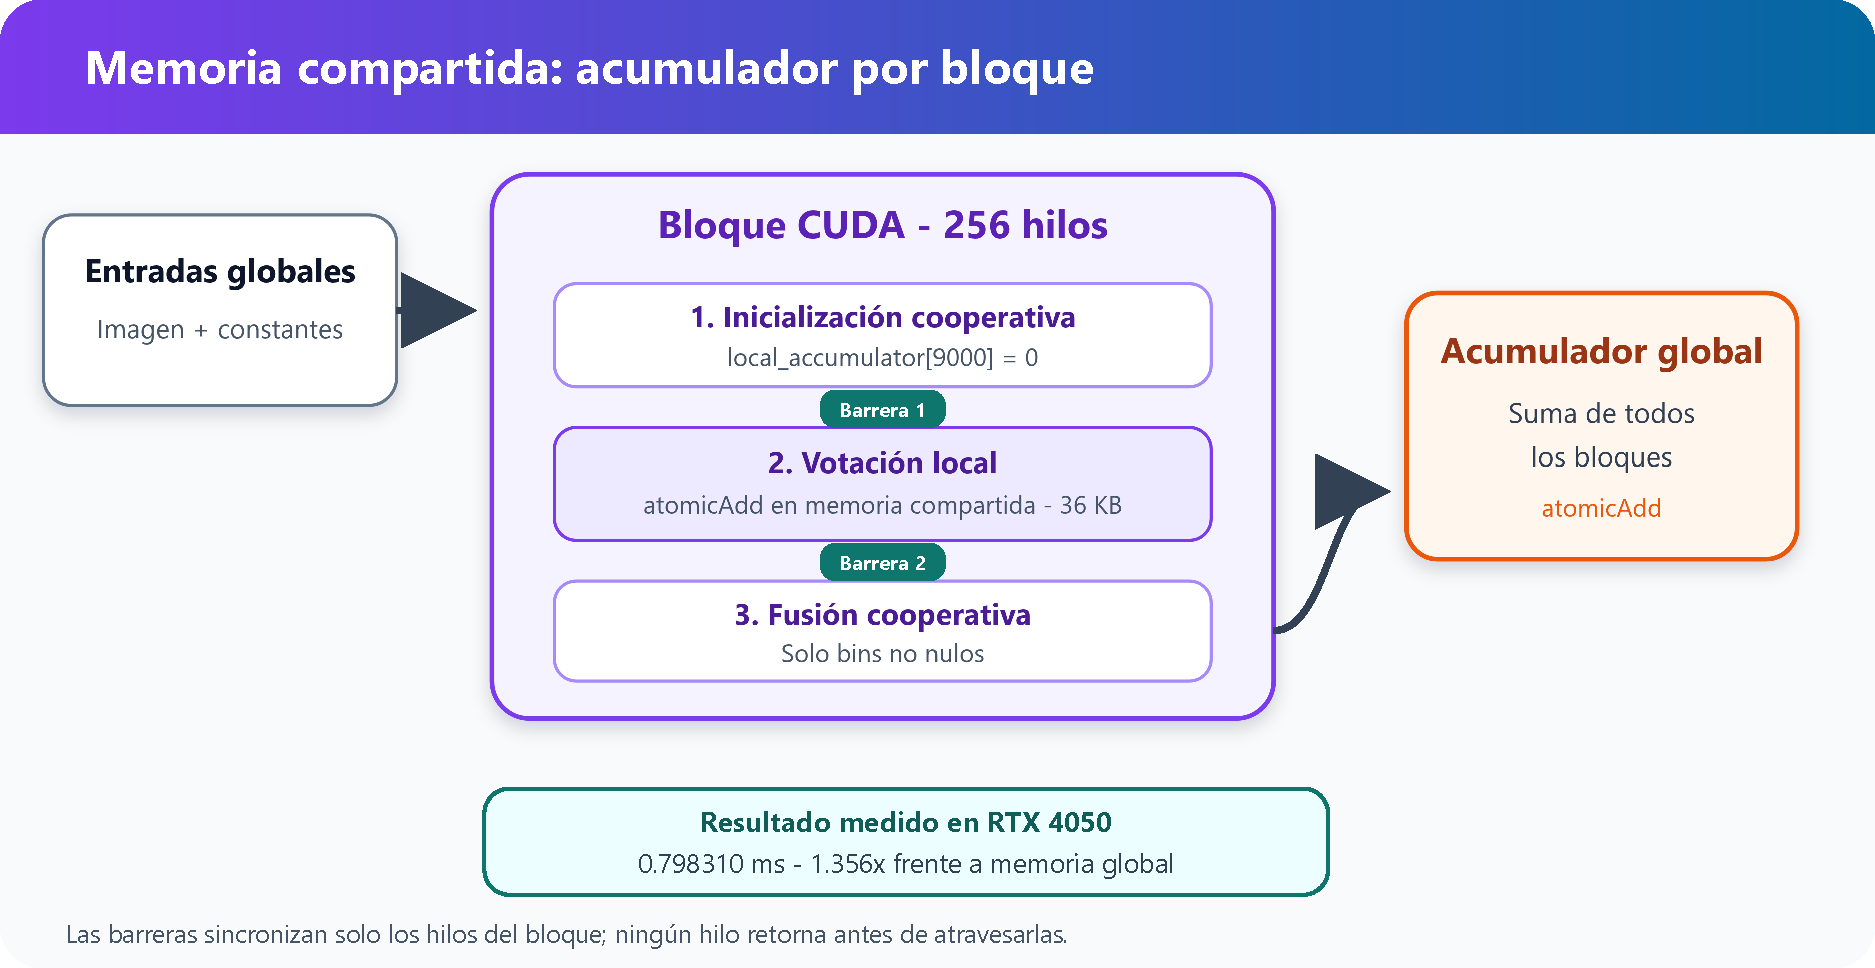
\includegraphics[width=\textwidth]{figures/memoria_compartida.pdf}
  \caption{Acumulador compartido por bloque y fusión global.}
  \label{fig:shared}
\end{figure}

La estrategia reduce la cantidad de atómicos globales, pero añade inicialización, dos barreras, atómicos compartidos y una fusión. Los 36 KB por bloque también pueden limitar la ocupación. El efecto neto debe determinarse mediante medición.

\section{Metodología experimental}

La corrida oficial utilizó una NVIDIA GeForce RTX 4050 Laptop GPU de 6 GB y capacidad de cómputo 8.9. El Toolkit fue CUDA 13.4 con \texttt{nvcc} 13.4.59 y el compilador host fue MSVC 19.44. La entrada \texttt{runway.pgm} tiene 800 por 600 píxeles, 138,406 píxeles activos y 12,456,540 votos de referencia.

Las variantes usan bloques de 256 hilos. Antes de registrar datos se ejecutaron dos calentamientos por kernel. Luego se realizaron diez mediciones por variante. Antes de cada lanzamiento se limpia el acumulador, pero \texttt{cudaMemset} permanece fuera del intervalo medido.

Dos CUDA Events se registran en el stream predeterminado. El evento final se sincroniza antes de calcular el tiempo con \texttt{cudaEventElapsedTime} \cite{cuda-events}. La medición excluye transferencias, referencia CPU, validación, selección de líneas y escritura PNG.

Se reportan media, mediana, desviación estándar, mínimo y máximo. Los valores individuales se conservan en \texttt{results/timings.csv}. Los tres acumuladores deben coincidir exactamente con CPU antes de aceptar sus tiempos.

\section{Resultados de rendimiento}

La Tabla~\ref{tab:summary} resume las treinta observaciones oficiales.

\begin{table}[H]
  \centering
  \caption{Resumen de tiempos del kernel, diez corridas por variante.}
  \label{tab:summary}
  \small
  \begin{tabular}{lrrrrrr}
    \toprule
    Variante & Media & Mediana & Desv. & Mín. & Máx. & Speedup \\
    \midrule
    Global & 1.082563 & 1.084368 & 0.003477 & 1.077248 & 1.087488 & 1.000x \\
    Constante & 1.074896 & 1.074704 & 0.003398 & 1.069056 & 1.081344 & 1.007x \\
    Compartida & 0.798310 & 0.798720 & 0.000502 & 0.797696 & 0.798720 & 1.356x \\
    \bottomrule
  \end{tabular}
\end{table}

\begin{figure}[H]
  \centering
  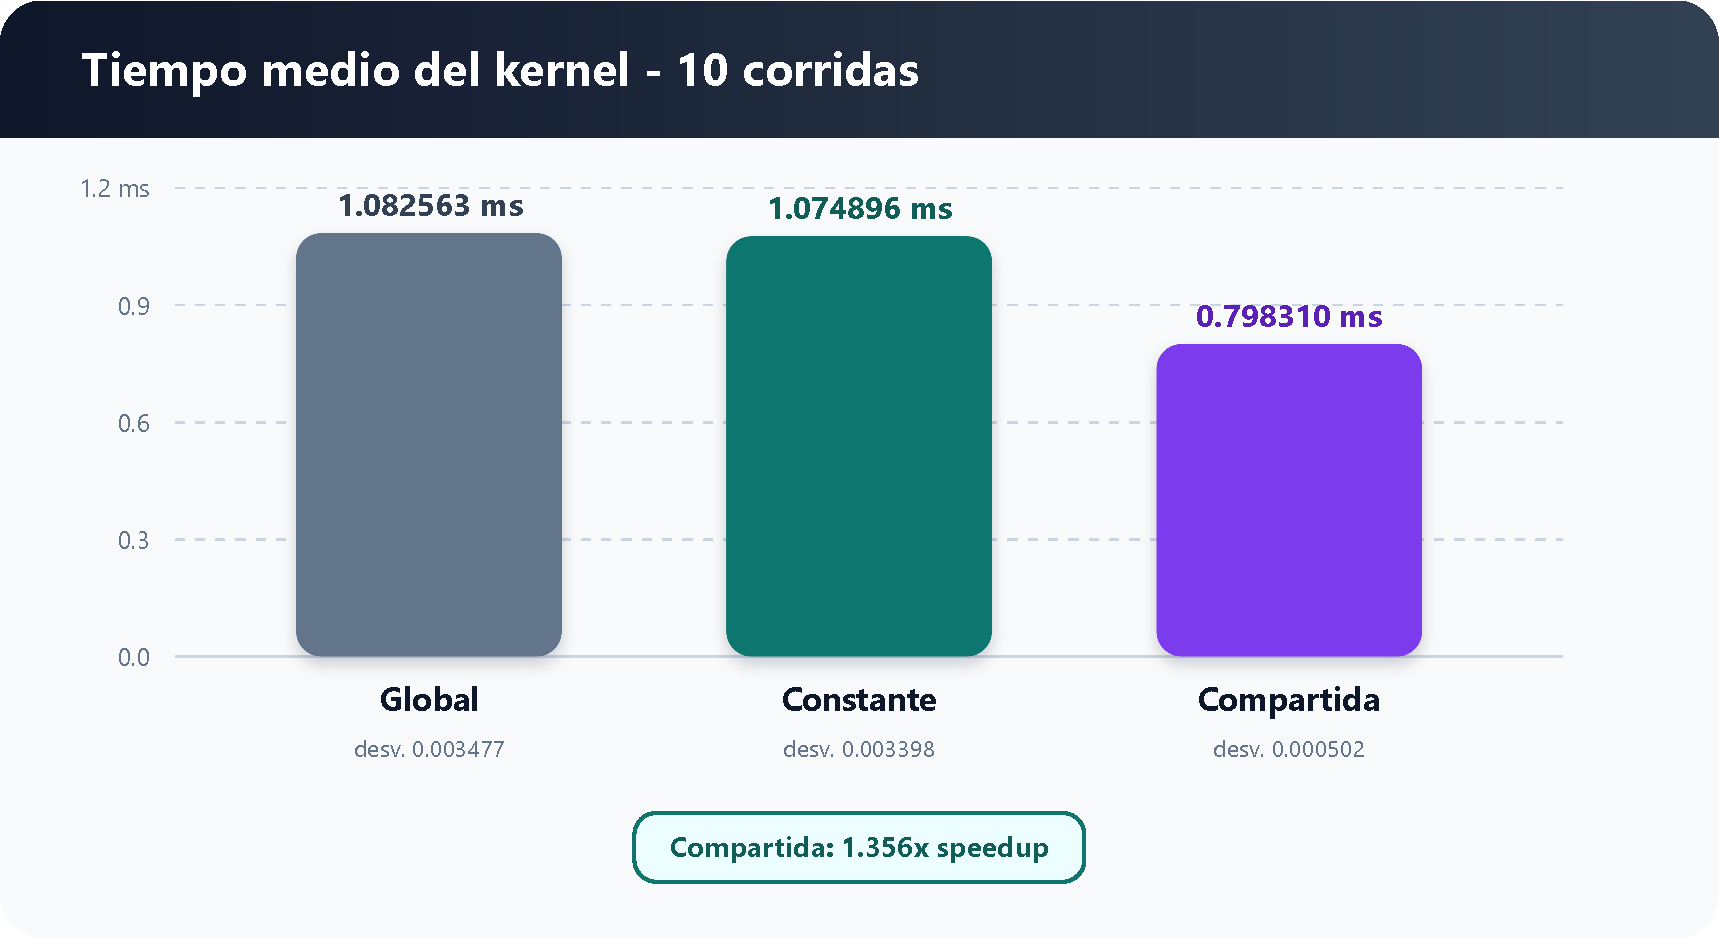
\includegraphics[width=0.92\textwidth]{figures/tiempos_kernel.pdf}
  \caption{Comparación de los tiempos medios del kernel.}
  \label{fig:times}
\end{figure}

Constante redujo el tiempo medio 0.71\% frente a Global. El patrón uniforme favorece el broadcast, pero las tablas son pequeñas y el acumulador continúa sujeto a atómicos globales.

Compartida redujo el tiempo medio 26.26\% y obtuvo un speedup de 1.3561x. En esta entrada, la disminución de actualizaciones globales compensó la inicialización local, las barreras y la fusión. También presentó la menor dispersión. El resultado corresponde a la RTX 4050 evaluada y no debe generalizarse sin repetir el experimento.

\section{Validación y pruebas}

Los acumuladores de Global, Constante y Compartida coincidieron exactamente con CPU para los 9,000 bins y 12,456,540 votos. Compute Sanitizer \texttt{memcheck} reportó cero errores. \texttt{racecheck} reportó cero peligros, cero errores y cero advertencias \cite{compute-sanitizer}.

CTest ejecutó siete pruebas y aprobó siete. La suite cubre entrada/salida, CLI y casos sintéticos cuyo total de votos puede calcularse antes de ejecutar la GPU.

\begin{table}[H]
  \centering
  \caption{Casos sintéticos principales.}
  \small
  \begin{tabularx}{\textwidth}{XrrX}
    \toprule
    Caso & Activos & Votos & Verificación \\
    \midrule
    Negra 8x8 & 0 & 0 & Sin picos \\
    Píxel único 9x9 & 1 & 90 & Tres acumuladores iguales \\
    Horizontal 17x17 & 17 & 1,530 & Pico en 90 grados \\
    Vertical 17x17 & 17 & 1,530 & Pico en 0 grados \\
    Cruce 17x17 & 33 & 2,970 & Orientaciones 0 y 90 \\
    Umbral 3x1 & 1 & 90 & Solo el valor 33 vota \\
    Sintética 7x5 & 15 & 1,350 & Último bloque incompleto \\
    \bottomrule
  \end{tabularx}
\end{table}

Las pruebas de imagen verifican PGM P2/P5, comentarios, escalado, firma PNG y rechazo de entradas truncadas o fuera de rango. Las pruebas CLI validan la ayuda y el rechazo de modos, conteos y rutas inválidas.

\section{Visualización de líneas}

El umbral de selección se calcula como:

\begin{equation}
  T = \mu + 2.4\sigma,
\end{equation}

donde $\mu$ y $\sigma$ corresponden a los 9,000 bins. Una supresión de máximos no locales usa radio 4 en $r$ y 3 en $\theta$. El tratamiento circular de $\theta$ respeta la equivalencia $(r,\theta)=(-r,\theta+180^\circ)$. La ejecución produjo seis máximos por encima de $T=3973.09$.

\begin{figure}[H]
  \centering
  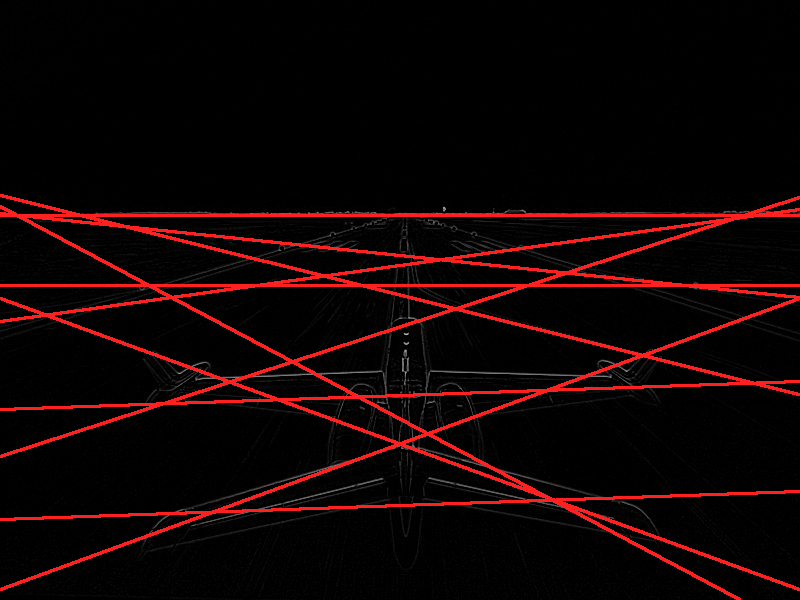
\includegraphics[width=\textwidth]{../results/runway_lines.png}
  \caption{Seis rectas detectadas sobre la imagen oficial.}
  \label{fig:output}
\end{figure}

Las líneas más fuertes incluyen el horizonte y bordes diagonales u horizontales de la pista y la aeronave. La selección visual ocurre después de medir y no altera el acumulador ni los tiempos del kernel.

\section{Conclusiones y recomendaciones}

La variante Compartida fue la más rápida, con 0.798310 ms de media y 0.000502 ms de desviación estándar. El acumulador por bloque redujo suficientemente la contención global para compensar su costo adicional. Sin embargo, sus 36 KB por bloque pueden reducir la ocupación, por lo que conviene revisar recursos y repetir las mediciones en cada arquitectura.

La memoria Constante produjo una mejora medible pero modesta de 0.71\%. Su uso coincide con el patrón de lectura uniforme de seno y coseno, aunque el pequeño tamaño de las tablas y los atómicos globales limitan el impacto total.

La corrección depende de operaciones atómicas, de las dos barreras bien ubicadas y de impedir retornos anticipados en el último bloque. La comparación exacta con CPU, los casos sintéticos y Compute Sanitizer aportan evidencia independiente de que los kernels conservan los votos y sincronizan correctamente.

Se recomienda mantener calentamientos, parámetros idénticos y un mínimo de diez corridas. Para caracterizar diferencias pequeñas, como la de Constante, conviene repetir sesiones en distintos momentos y reportar dispersión. Cualquier cambio de GPU, imagen, umbral o discretización debe documentarse y medirse de nuevo.

\clearpage
\section{Referencias}

\begin{thebibliography}{9}
  \bibitem{duda-hart}
  R. O. Duda y P. E. Hart,
  ``Use of the Hough Transformation to Detect Lines and Curves in Pictures'',
  \emph{Communications of the ACM}, vol. 15, núm. 1, pp. 11--15, 1972.
  \url{https://doi.org/10.1145/361237.361242}

  \bibitem{cuda-guide}
  NVIDIA Corporation,
  \emph{CUDA C++ Programming Guide}, espacios de memoria y sincronización.
  \url{https://docs.nvidia.com/cuda/cuda-programming-guide/}

  \bibitem{cuda-events}
  NVIDIA Corporation,
  \emph{CUDA Runtime API: Event Management}.
  \url{https://docs.nvidia.com/cuda/cuda-runtime-api/group__CUDART__EVENT.html}

  \bibitem{compute-sanitizer}
  NVIDIA Corporation,
  \emph{Compute Sanitizer Documentation}.
  \url{https://docs.nvidia.com/compute-sanitizer/}
\end{thebibliography}

\appendix
\section{Material suplementario}

\subsection{Archivos principales}

\begin{itemize}
  \item \texttt{src/hough.cu}: referencia CPU, kernels, medición, validación y dibujo.
  \item \texttt{common/image\_io.cpp}: lectura PGM y escritura PNG.
  \item \texttt{results/timings.csv}: treinta observaciones experimentales.
  \item \texttt{results/detected\_lines.csv}: parámetros y votos de las seis líneas.
  \item \texttt{results/run\_metadata.txt}: configuración de la corrida oficial.
  \item \texttt{tests/}: casos de I/O, CLI y regresión GPU.
  \item \texttt{BITACORA.md}: entorno, protocolo, mediciones y comprobaciones.
\end{itemize}

\subsection{Criterios de aceptación}

\begin{itemize}
  \item Los tres acumuladores GPU coinciden exactamente con CPU.
  \item Cada variante tiene diez mediciones posteriores a dos calentamientos.
  \item CTest aprueba siete de siete pruebas.
  \item Memcheck no reporta accesos inválidos y racecheck no reporta peligros.
  \item La salida PNG se abre correctamente y muestra las rectas seleccionadas.
  \item El programa libera memoria, destruye eventos y reinicia el dispositivo.
\end{itemize}

\subsection{Trazabilidad}

La corrida oficial se realizó el 25 de octubre de 2026 con CUDA 13.4.59 y MSVC 19.44. La línea base técnica validada fue \texttt{a5955e4}; el primer paquete documental final se generó desde \texttt{cb28172}. Entre ambos commits no cambiaron los kernels, archivos de construcción ni datos oficiales de medición. La revisión documental del 7 de noviembre se mantuvo local para aprobación antes de regenerar los paquetes.

\section{Análisis de complejidad y memoria}

Sea $P$ la cantidad total de píxeles, $P_a$ la cantidad de píxeles activos, $A$ la cantidad de ángulos y $B$ el número de bins del acumulador. En la entrada oficial:

\[
P = 800\times600 = 480{,}000, \qquad P_a = 138{,}406,
\]

\[
A = 90, \qquad B = 90\times100 = 9{,}000.
\]

El trabajo de votación es $O(P_aA)$, además del recorrido inicial de los píxeles. La cantidad exacta de votos de la imagen oficial es:

\[
138{,}406\times90 = 12{,}456{,}540.
\]

La referencia CPU y los kernels Global y Constante realizan conceptualmente esos votos sobre un acumulador común. Compartida agrega el costo de inicializar y fusionar un acumulador de $B$ elementos por bloque. En el peor caso esa etapa añade $O(N_bB)$ operaciones, donde $N_b$ es el número de bloques, aunque la fusión omite bins con valor cero.

Con bloques de 256 hilos, la imagen oficial usa 1,875 bloques. El tamaño de imagen es múltiplo exacto de 256; por ello los casos sintéticos incluyen una imagen de 7 por 5 para comprobar explícitamente un último bloque incompleto.

\begin{table}[H]
  \centering
  \caption{Huella de los datos principales.}
  \begin{tabularx}{\textwidth}{XrrX}
    \toprule
    Recurso & Elementos & Tamaño & Ubicación principal \\
    \midrule
    Imagen PGM & 480,000 bytes & 468.75 KiB & Global \\
    Acumulador & 9,000 enteros & 36,000 bytes & Global \\
    Seno y coseno & 180 flotantes & 720 bytes & Global o Constante \\
    Acumulador local & 9,000 enteros & 36,000 bytes & Compartida por bloque \\
    \bottomrule
  \end{tabularx}
\end{table}

El acumulador compartido consume la mayor parte de los recursos explícitos por bloque. Esta decisión reduce contención, pero puede limitar la cantidad de bloques residentes simultáneamente en un multiprocesador.

\section{Jerarquía de memoria y atomicidad}

La comparación no pretende afirmar que un acceso denominado ``global'' ignore las cachés del hardware. Los nombres de las variantes identifican dónde se declaran y actualizan explícitamente los datos que cambian entre experimentos.

En Global, las tablas y el acumulador residen en memoria global. Las tablas presentan reutilización temporal, pero cada voto todavía necesita coordinarse con todos los bloques. En Constante, las tablas pasan a un espacio de solo lectura adecuado para el patrón uniforme por warp. El acumulador no cambia de ubicación, por lo que la optimización cubre solo una parte del kernel.

En Compartida, la mayoría de los votos se agrupa dentro del bloque. Las operaciones atómicas compartidas coordinan hilos del mismo bloque; la fusión final usa atómicos globales para combinar bloques. La estrategia reduce la frecuencia de actualizaciones globales, pero no las elimina.

\subsection{Razón de las operaciones atómicas}

Si dos hilos leen el mismo contador, calculan por separado el valor incrementado y escriben sin atomicidad, una actualización puede sobrescribir la otra. \texttt{atomicAdd} convierte la lectura, suma y escritura en una operación indivisible desde la perspectiva de los hilos participantes.

\subsection{Razón de las barreras}

La primera barrera separa la inicialización de la votación. La segunda separa la votación de la fusión. Una barrera de bloque exige que todos los hilos activos alcancen el mismo punto. Por eso un hilo fuera de los límites de la imagen no retorna anticipadamente en la versión Compartida.

\section{Detalle de las treinta mediciones}

\begin{longtable}{rrrr}
  \caption{Tiempos individuales del kernel en milisegundos.}\\
  \toprule
  Corrida & Global & Constante & Compartida \\
  \midrule
  \endfirsthead
  \toprule
  Corrida & Global & Constante & Compartida \\
  \midrule
  \endhead
  1 & 1.078272 & 1.073152 & 0.798720 \\
  2 & 1.084416 & 1.074176 & 0.798720 \\
  3 & 1.084416 & 1.078272 & 0.797696 \\
  4 & 1.082368 & 1.081344 & 0.797696 \\
  5 & 1.084320 & 1.071104 & 0.797696 \\
  6 & 1.087488 & 1.077248 & 0.798720 \\
  7 & 1.077248 & 1.069056 & 0.798720 \\
  8 & 1.077248 & 1.073152 & 0.798720 \\
  9 & 1.084416 & 1.076224 & 0.798720 \\
  10 & 1.085440 & 1.075232 & 0.797696 \\
  \midrule
  Media & 1.082563 & 1.074896 & 0.798310 \\
  Desv. estándar & 0.003477 & 0.003398 & 0.000502 \\
  \bottomrule
\end{longtable}

El coeficiente de variación, calculado como desviación estándar dividida entre la media, fue aproximadamente 0.321\% para Global, 0.316\% para Constante y 0.063\% para Compartida. Las tres series presentan poca dispersión; Compartida fue la más estable en esta sesión.

La diferencia media entre Global y Constante fue 0.007667 ms. Aunque aparece de forma consistente en el promedio, es pequeña en términos absolutos y conviene confirmarla con sesiones adicionales si se quiere generalizar. La diferencia entre Global y Compartida fue 0.284253 ms, notablemente mayor que la dispersión observada.

\section{Reproducibilidad y límites de la medición}

La medición aísla el kernel para estudiar la jerarquía de memoria. El intervalo comienza después de limpiar el acumulador y termina cuando se completa el lanzamiento medido. No incluye lectura del PGM, asignación de buffers, transferencias host-device, referencia CPU, comparación, selección de máximos ni escritura PNG.

Este límite debe conservarse al interpretar los datos: los tiempos describen el costo del kernel, no la latencia completa de la aplicación. Una comparación de extremo a extremo requeriría medir por separado carga, copias, cómputo y salida.

\subsection{Procedimiento reproducible}

\begin{enumerate}
  \item Conectar el equipo a corriente y usar un perfil de alto rendimiento.
  \item Cerrar cargas intensivas de GPU y registrar \texttt{nvidia-smi}.
  \item Compilar en modo optimizado con la misma arquitectura CUDA.
  \item Ejecutar dos calentamientos y diez corridas por variante.
  \item Confirmar las tres validaciones CPU-GPU.
  \item Guardar CSV, metadatos, PNG y registros de sanitización.
\end{enumerate}

Comando usado en Windows:

\begin{lstlisting}[language={}]
powershell.exe -NoProfile -ExecutionPolicy Bypass \
  -File .\scripts\run_benchmarks.ps1 \
  -Executable ".\hough.exe" -Runs 10 -Warmup 2
\end{lstlisting}

Para comparar otra GPU se deben conservar la imagen, los parámetros, la discretización y la definición del intervalo medido. El modelo de GPU, Toolkit, compilador host, controlador y perfil de energía deben registrarse de nuevo.

\section{Cobertura detallada de pruebas}

Las pruebas se diseñaron para separar errores de E/S, CLI, geometría, umbral y sincronización. Cada caso GPU ejecuta las tres variantes y exige igualdad exacta con CPU.

\begin{table}[H]
  \centering
  \caption{Relación entre riesgo y prueba.}
  \small
  \begin{tabularx}{\textwidth}{X X X}
    \toprule
    Riesgo & Caso & Evidencia esperada \\
    \midrule
    Votos espurios & Negra 8x8 & Cero píxeles y cero votos \\
    Error de conteo mínimo & Píxel 9x9 & 90 votos \\
    Orientación incorrecta & Horizontal/vertical & Picos en 90/0 grados \\
    Pérdida de una intersección & Cruce 17x17 & Ambas orientaciones \\
    Comparación incorrecta del umbral & Valores 31, 32 y 33 & Solo 33 vota \\
    Retorno antes de barrera & Sintética 7x5 & Bloque incompleto válido \\
    Lectura insegura & PGM truncado/fuera de rango & Rechazo controlado \\
    Argumentos inválidos & CLI & Código de error \\
    \bottomrule
  \end{tabularx}
\end{table}

\texttt{memcheck} busca accesos fuera de rango y uso inválido de memoria. \texttt{racecheck} analiza peligros de acceso en memoria compartida. Sus tiempos incluyen instrumentación y no deben compararse con los tiempos oficiales.

\section{Retos, amenazas a la validez y trabajo futuro}

\subsection{Retos encontrados}

El primer reto fue preparar un entorno Windows compatible: \texttt{nvcc} necesita el compilador host de MSVC y sus variables de entorno. El README documenta el uso de la consola x64 y la carga de \texttt{VsDevCmd.bat}.

El segundo reto fue sincronizar el acumulador compartido sin excluir hilos sobrantes. La solución separó la condición de votación de las barreras, de modo que todos los hilos del bloque atraviesan ambas sincronizaciones.

El tercer reto fue evitar líneas duplicadas en la salida. Se combinó un umbral estadístico con supresión de máximos no locales y tratamiento circular del ángulo.

\subsection{Amenazas a la validez}

Las mediciones provienen de una sola GPU, una sola imagen y una sesión oficial. La diferencia de Constante es pequeña y puede ser sensible a frecuencia, temperatura o actividad del sistema. La entrada también determina la distribución de contención en los bins.

El tiempo de kernel no representa la aplicación completa. Además, los 36 KB compartidos pueden producir una ocupación distinta en otra arquitectura. Estas limitaciones no invalidan la comparación interna, pero restringen su generalización.

\subsection{Trabajo futuro}

Se propone repetir sesiones en varias GPU, estudiar ocupación con herramientas de perfilado, variar la densidad de píxeles activos y comparar diferentes cantidades de bins. También sería útil medir el flujo completo y separar transferencias, kernel y posprocesamiento.

\section{Correspondencia con el enunciado}

\begin{table}[H]
  \centering
  \caption{Trazabilidad de requisitos y evidencia.}
  \begin{tabularx}{\textwidth}{X X X}
    \toprule
    Requisito & Implementación & Evidencia \\
    \midrule
    Global funcional & Kernel base y \texttt{atomicAdd} & Validación y tiempos \\
    CUDA Events & Eventos antes/después del kernel & \texttt{timings.csv} \\
    Coordenadas centradas & Cálculo desde \texttt{global\_id} & Secciones 2 y 3 \\
    Imagen con líneas & Umbral, NMS y escritor PNG & \texttt{runway\_lines.png} \\
    Memoria Constante & Símbolos y \texttt{cudaMemcpyToSymbol} & Figura 1 y resultados \\
    Memoria Compartida & \texttt{local\_accumulator} y dos barreras & Figura 2 y racecheck \\
    Diez tiempos por versión & Treinta observaciones & Tabla de mediciones \\
    Liberación de recursos & RAII y \texttt{cudaDeviceReset} & Código final \\
    Presentación & HTML offline de 11 diapositivas & \texttt{presentacion.html} \\
    \bottomrule
  \end{tabularx}
\end{table}

\end{document}
